\documentclass[12pt]{beamer}
\usepackage{beamerthemeHannover, graphicx, clrscode, amsmath, amssymb, multicol}
\setbeamercolor{sidebar}{use=structure,bg=gray!20!red!60!white}
\title{Getting Involved With Rakudo \\ \small{ (A Flavor of Perl 6) } }
\author[Duke Leto]{Jonathan "Duke" Leto}
\date{}

\begin{document}

\frame{
    \titlepage
    \begin{center}
        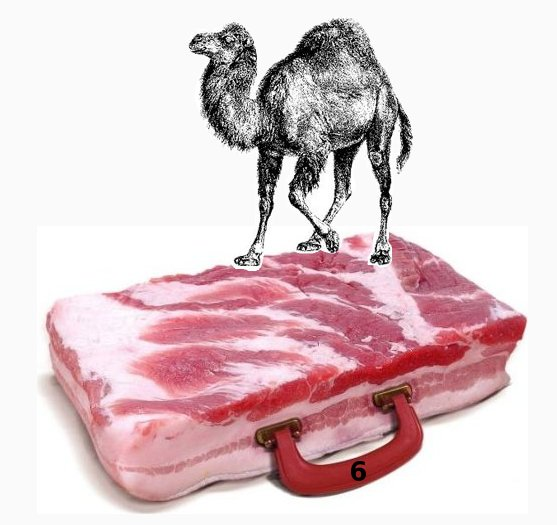
\includegraphics[width=4.57cm, height=4.25cm]{perl6bacon}
    \end{center}
}

\section{What is Perl 6?}
\frame{
    \frametitle{Flavors of Perl 6}
    \begin{center}
        \begin{itemize}
            \item Rakudo - Parrot
            \item Pugs - Haskell
            \item SMOP - C+DSLs
            \item Elf - Ruby
            \item STD.pm - Larry's Implementation in Perl 6 (gimme5)
            \item v6.pm - Source filter for Perl 5
            \item others ...
        \end{itemize}
    \end{center}
}

\frame{
    \frametitle{What is Rakudo?}
    \small{ The Way Of The Camel  = "Rakuda-do" $\implies$ Rakudo, which happens to mean "paradise" in Japanese. }

    \begin{center}
        \begin{itemize}
            \item Perl 6 implementation on the Parrot Virtual Machine
            \item Still lives in \begin{bf}languages/perl6\end{bf} directory of Parrot
            \item Fierce development in the last few weeks
            \item Aiming to be the first production Perl 6 implementation
            \item 1.0 ? Sometime before Xmas
        \end{itemize}
    \end{center}
}

\frame{
    \frametitle{ Resources }
    \begin{center}
        \begin{itemize}
           \item http://rakudo.org
           \item http://parrot.org
           \item http://perlsphere.net
        \end{itemize}
    \end{center}
}

\end{document}
